\documentclass[tikz]{standalone}

\begin{document}
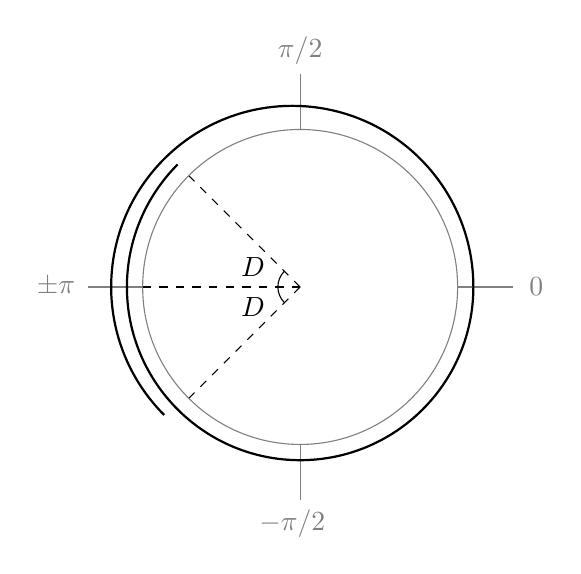
\begin{tikzpicture}

% The circle itself
\draw[color=gray] (0,0) circle (2);

% The markings
\draw[color=gray] (2,0) -- (2.7,0);
\draw[color=gray] (0,2) -- (0,2.7);
\draw[color=gray] (0,-2) -- (0,-2.7);
\draw[color=gray] (-2,0) -- (-2.7,0);

% The labels
\node[color=gray] at (3,0) {\(0\)};
\node[color=gray] at (0,3) {\(\pi/2\)};
\node[color=gray] at (-.1,-3) {\(-\pi/2\)};
\node[color=gray] at (-3.1,0) {\(\pm\pi\)};

% The covers
\draw[color=black,thick] (2.2,0) arc (0:225:2.3);
\draw[color=black,thick] (2.2,0) arc (0:-225:2.2);

% The angles
\draw[color=black, dashed] (-2,0) -- (0,0);
\draw[color=black, dashed] (0,0) -- (-1.41,1.41);
\draw[color=black, dashed] (0,0) -- (-1.41,-1.41);

% The angle circle
\draw[color=black] (-.2,.2) arc (135:225:.282);

% The angle labels
\node at (-.6,.25) {\(D\)};
\node at (-.6,-.25) {\(D\)};

\end{tikzpicture}
\end{document}
